%!TEX root = ../dokumentation.tex

\chapter{Softwaretechnik}

\section{Softwarepakete}

\section{Entwicklungsumgebung}

\section{Emulation}

Die App wurde sowohl im Simulator, als auch auf zwei physischen Endgeräten getestet.
Die verwendeten Geräte umfassen:

iOS:
-	Simulator: iPhone SE (3rd Generation), iOS 17.0
Die iOS-Simulation wurde mit dem SimulatorKit von Apple in der Version 15.0.1 (1015.2) ausgeführt.

Android:
-	Simulator: Pixel 3a, Api-Version 27, Android 8.1 (Oreo)

\begin{figure}[H]
    \centering
    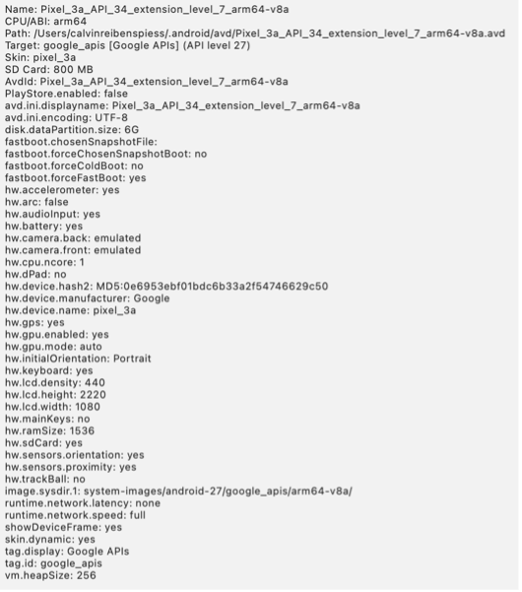
\includegraphics[width=0.8\textwidth]{images/android_emulator_reibenspiess.png}
    \caption{Einstellungen des Android-Emulators von Calvin Reibenspieß.}
    \label{branding}
  \end{figure}

\section{Hardware}

-	iPhone 12 Pro, iOS 16.1.2
IMEI: 35 861174 3743835